\documentclass{InsightArticle}

\usepackage[dvips]{graphicx}
\usepackage{float}
\usepackage{subfigure}

\usepackage[dvips,
bookmarks,
bookmarksopen,
backref,
colorlinks,linkcolor={blue},citecolor={blue},urlcolor={blue},
]{hyperref}

\title{Closed Loop Simplification}

% 
% NOTE: This is the last number of the "handle" URL that 
% The Insight Journal assigns to your paper as part of the
% submission process. Please replace the number "1338" with
% the actual handle number that you get assigned.
%
\newcommand{\IJhandlerIDnumber}{3302}

% Increment the release number whenever significant changes are made.
% The author and/or editor can define 'significant' however they like.
\release{0.00}

% At minimum, give your name and an email address.  You can include a
% snail-mail address if you like.

\author{David Doria}
\authoraddress{Rensselaer Polytechnic Institute}


\begin{document}

\IJhandlefooter{\IJhandlerIDnumber}


\ifpdf
\else
   %
   % Commands for including Graphics when using latex
   % 
   \DeclareGraphicsExtensions{.eps,.jpg,.gif,.tiff,.bmp,.png}
   \DeclareGraphicsRule{.jpg}{eps}{.jpg.bb}{`convert #1 eps:-}
   \DeclareGraphicsRule{.gif}{eps}{.gif.bb}{`convert #1 eps:-}
   \DeclareGraphicsRule{.tiff}{eps}{.tiff.bb}{`convert #1 eps:-}
   \DeclareGraphicsRule{.bmp}{eps}{.bmp.bb}{`convert #1 eps:-}
   \DeclareGraphicsRule{.png}{eps}{.png.bb}{`convert #1 eps:-}
\fi


\maketitle


\ifhtml
\chapter*{Front Matter\label{front}}
\fi

\begin{abstract}
\noindent

This document presents an implementation of Moore Neighbor Tracing - an algorithm to find an ordered outline of a blob in an image. The algorithm also works for images already containing contours (non-filled blobs) in that it assigns an ordering to the contour pixels.

An excellent tutorial on Moore Neighbor Tracing is provided here:
http://www.imageprocessingplace.com/downloads_V3/root_downloads/tutorials/contour_tracing_Abeer_George_Ghuneim/moore.html


The code is available here:
https://github.com/daviddoria/MooreTracing

\end{abstract}

\IJhandlenote{\IJhandlerIDnumber}

\tableofcontents
%%%%%%%%%%%%%%%%%%%%
\section{Introduction}
This document presents an implementation of Moore Neighbor Tracing - an algorithm to find an ordered outline of a blob in an image. The algorithm also works for images already containing contours (non-filled blobs) in that it assigns an ordering to the contour pixels.

An excellent tutorial on Moore Neighbor Tracing is provided here:
http://www.imageprocessingplace.com/downloads_V3/root_downloads/tutorials/contour_tracing_Abeer_George_Ghuneim/moore.html

This particular implementation is designed to be used with a ``label image'', typically the output of a pipeline consisting of one of many filters that produces an itkLabelMap (e.g. itkBinaryImageToLabelMapFilter) followed by a itkLabelMapToLabelImageFilter. Therefore, since we are looking to order the pixels in an already-known-to-be closed blob or contour, the termination criterion that has been implemented is returning to the starting pixel. Moore Neighbor Tracing can also be used with other stopping criteria to order pixels of open contours.

The code is available here:
https://github.com/daviddoria/MooreTracing

%%%%%%%%%%%%%%%%%%%%
\section{Algorithm}
The algorithm proceeds as follows:

Initialization:
\begin{enumerate}
\item Start on a boundary pixel. This can be found simply using a raster scan of the image and looking for the first non-background pixel.
{enumerate}
\begin{enumerate}
  \item Start on a boundary pixel. This can be found simply using a raster scan of the image and looking for the first non-background pixel.
 \item Record the pixel from which you ``entered'' the contour pixel.
 \item Traverse the 8-connected neighbors in a clockwise manner, looking for another non-background pixel.
\end{enumerate}

\subsection{Straightness Test}
\label{sec:Algorithm:StraightnessTest}
Edges from the complete graph are actually created only if they approximate the points on the input contour reasonably well, to a specified threshold. Figure \ref{fig:Straightness} represents the straightness calculation graphically.
\begin{figure}[H]
  \centering
  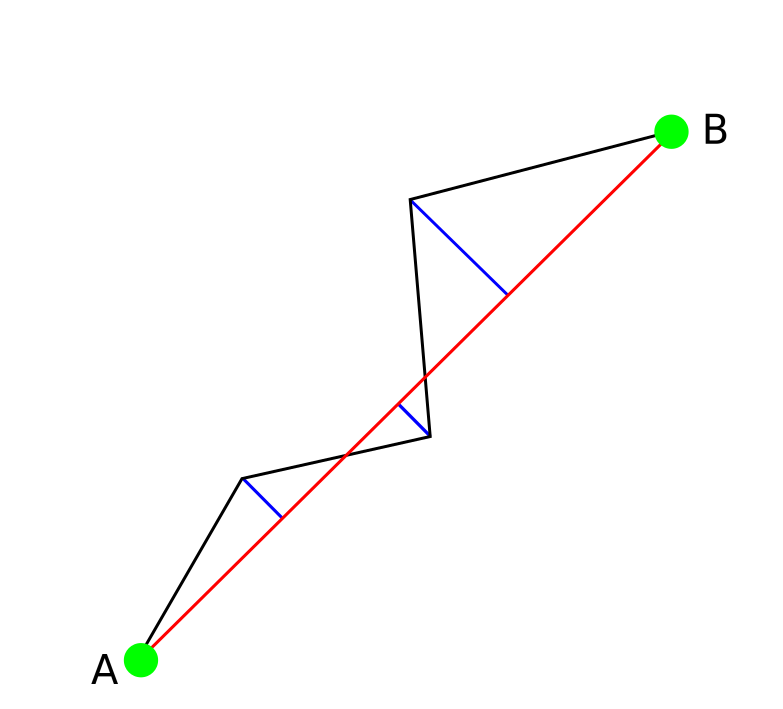
\includegraphics[width=0.3\linewidth]{images/straightness}
  \caption{The straightness computation of a proposed edge between vertices A and B. Black: the original contour. Red: the proposed edge. Blue: the perpendicular line from each vertex on the contour boundary between A and B to the proposed edge. The length of these lines are averaged to obtain the ``straightness'' of the line.}
  \label{fig:Straightness}
\end{figure}

Figure \ref{fig:PotentialEdges} shows the edges that were created using various straightness thresholds.
\begin{figure}[H]
\centering
\subfigure[Input contour.]
  {
  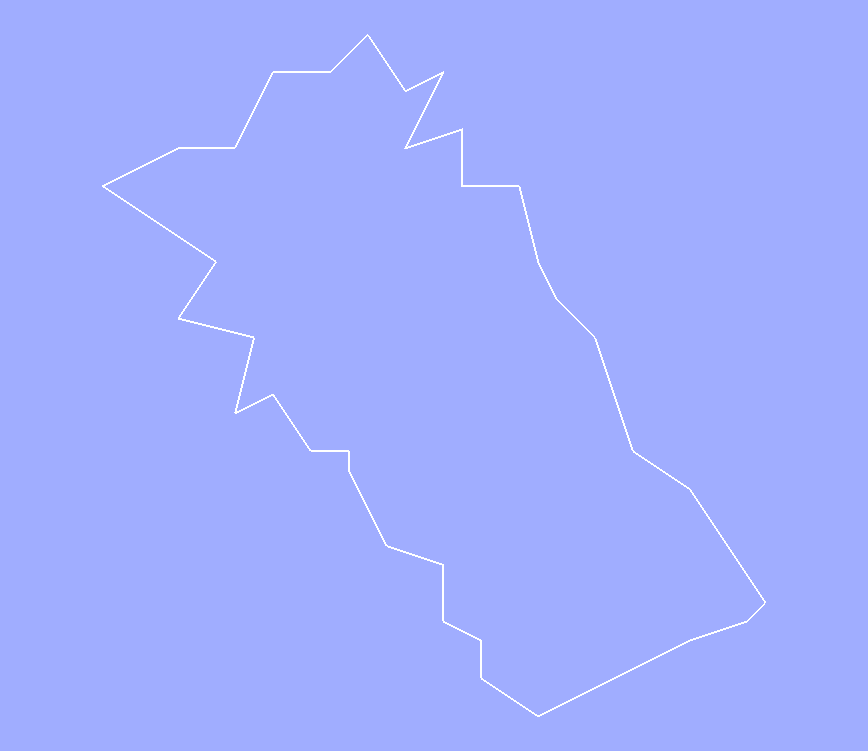
\includegraphics[width=0.22\linewidth]{images/noisy}
  \label{fig:PotentialEdges:input}
  }
\subfigure[PotentialEdges with StraightnessThreshold = 1.]
  {
  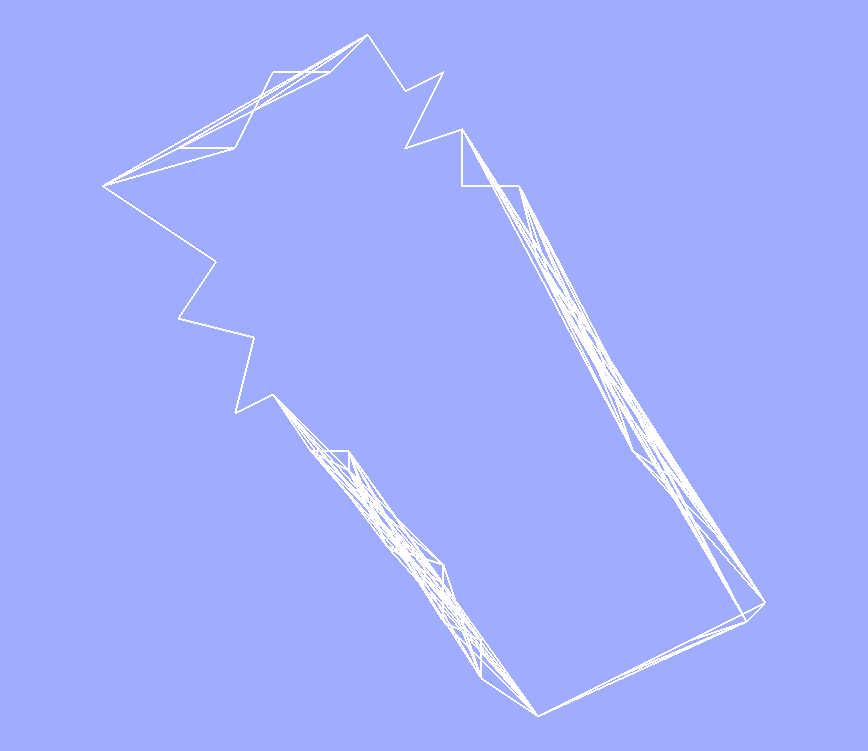
\includegraphics[width=0.22\linewidth]{images/noisyPotentialEdges_1}
  \label{fig:PotentialEdges:1}
  }
\subfigure[PotentialEdges with StraightnessThreshold = 5.]
  {
  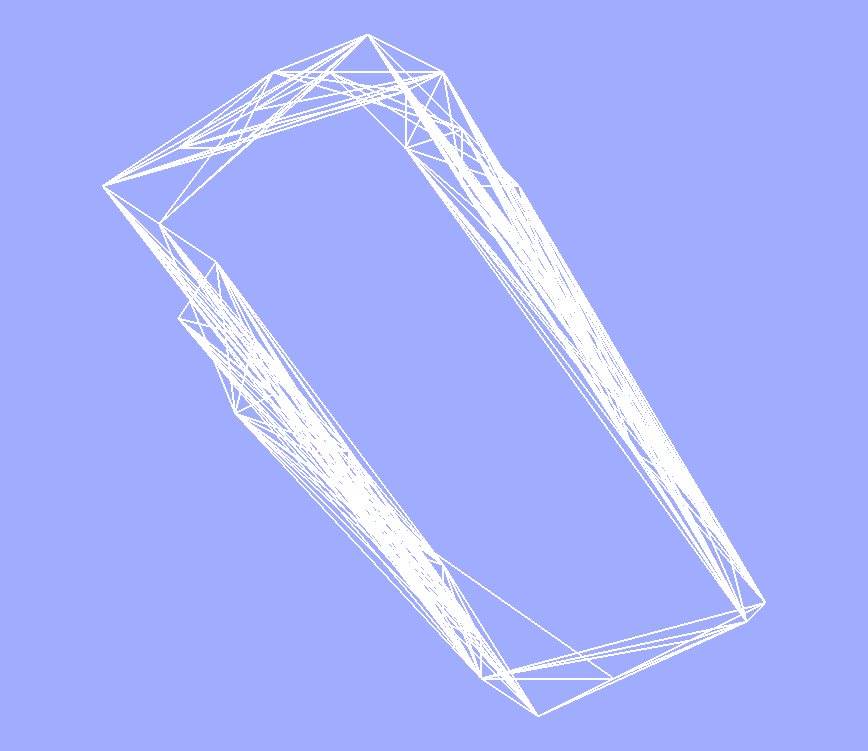
\includegraphics[width=0.22\linewidth]{images/noisyPotentialEdges_5}
  \label{fig:PotentialEdges:5}
  }
\subfigure[PotentialEdges with StraightnessThreshold = 10.]
  {
  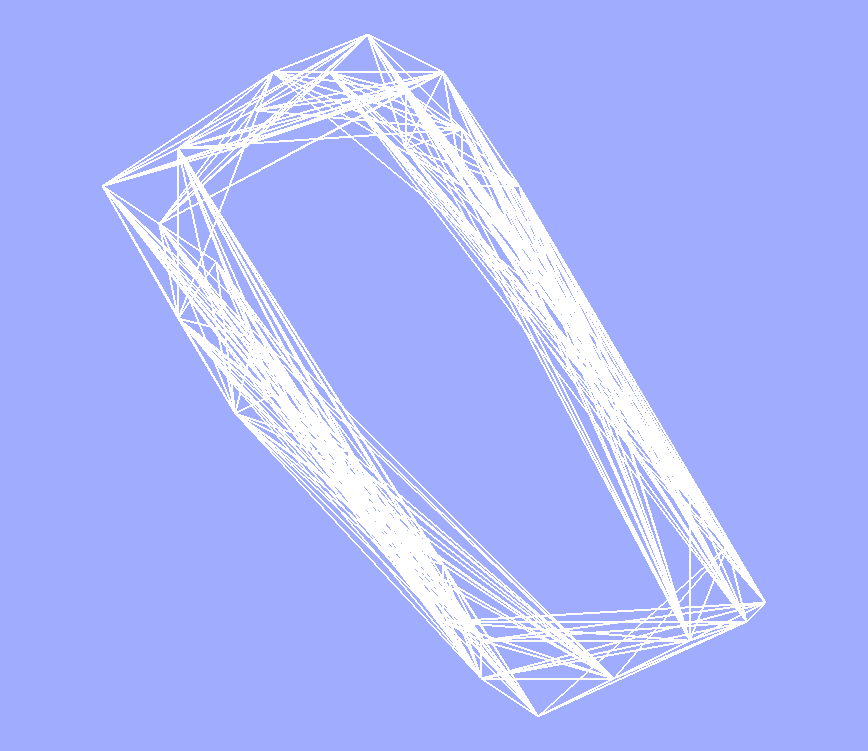
\includegraphics[width=0.22\linewidth]{images/noisyPotentialEdges_10}
  \label{fig:PotentialEdges:10}
  }
\caption{Images of the potential edges with StraightnessThreshold = 1, 5, and 10.}
\label{fig:PotentialEdges}
\end{figure}

\subsection{``Double Graph''}
\label{sec:Algorithm:DoubleLoopEdges}
Consider the graph shown in Figure \ref{fig:TwoLoops1}.

\begin{figure}[H]
  \centering
  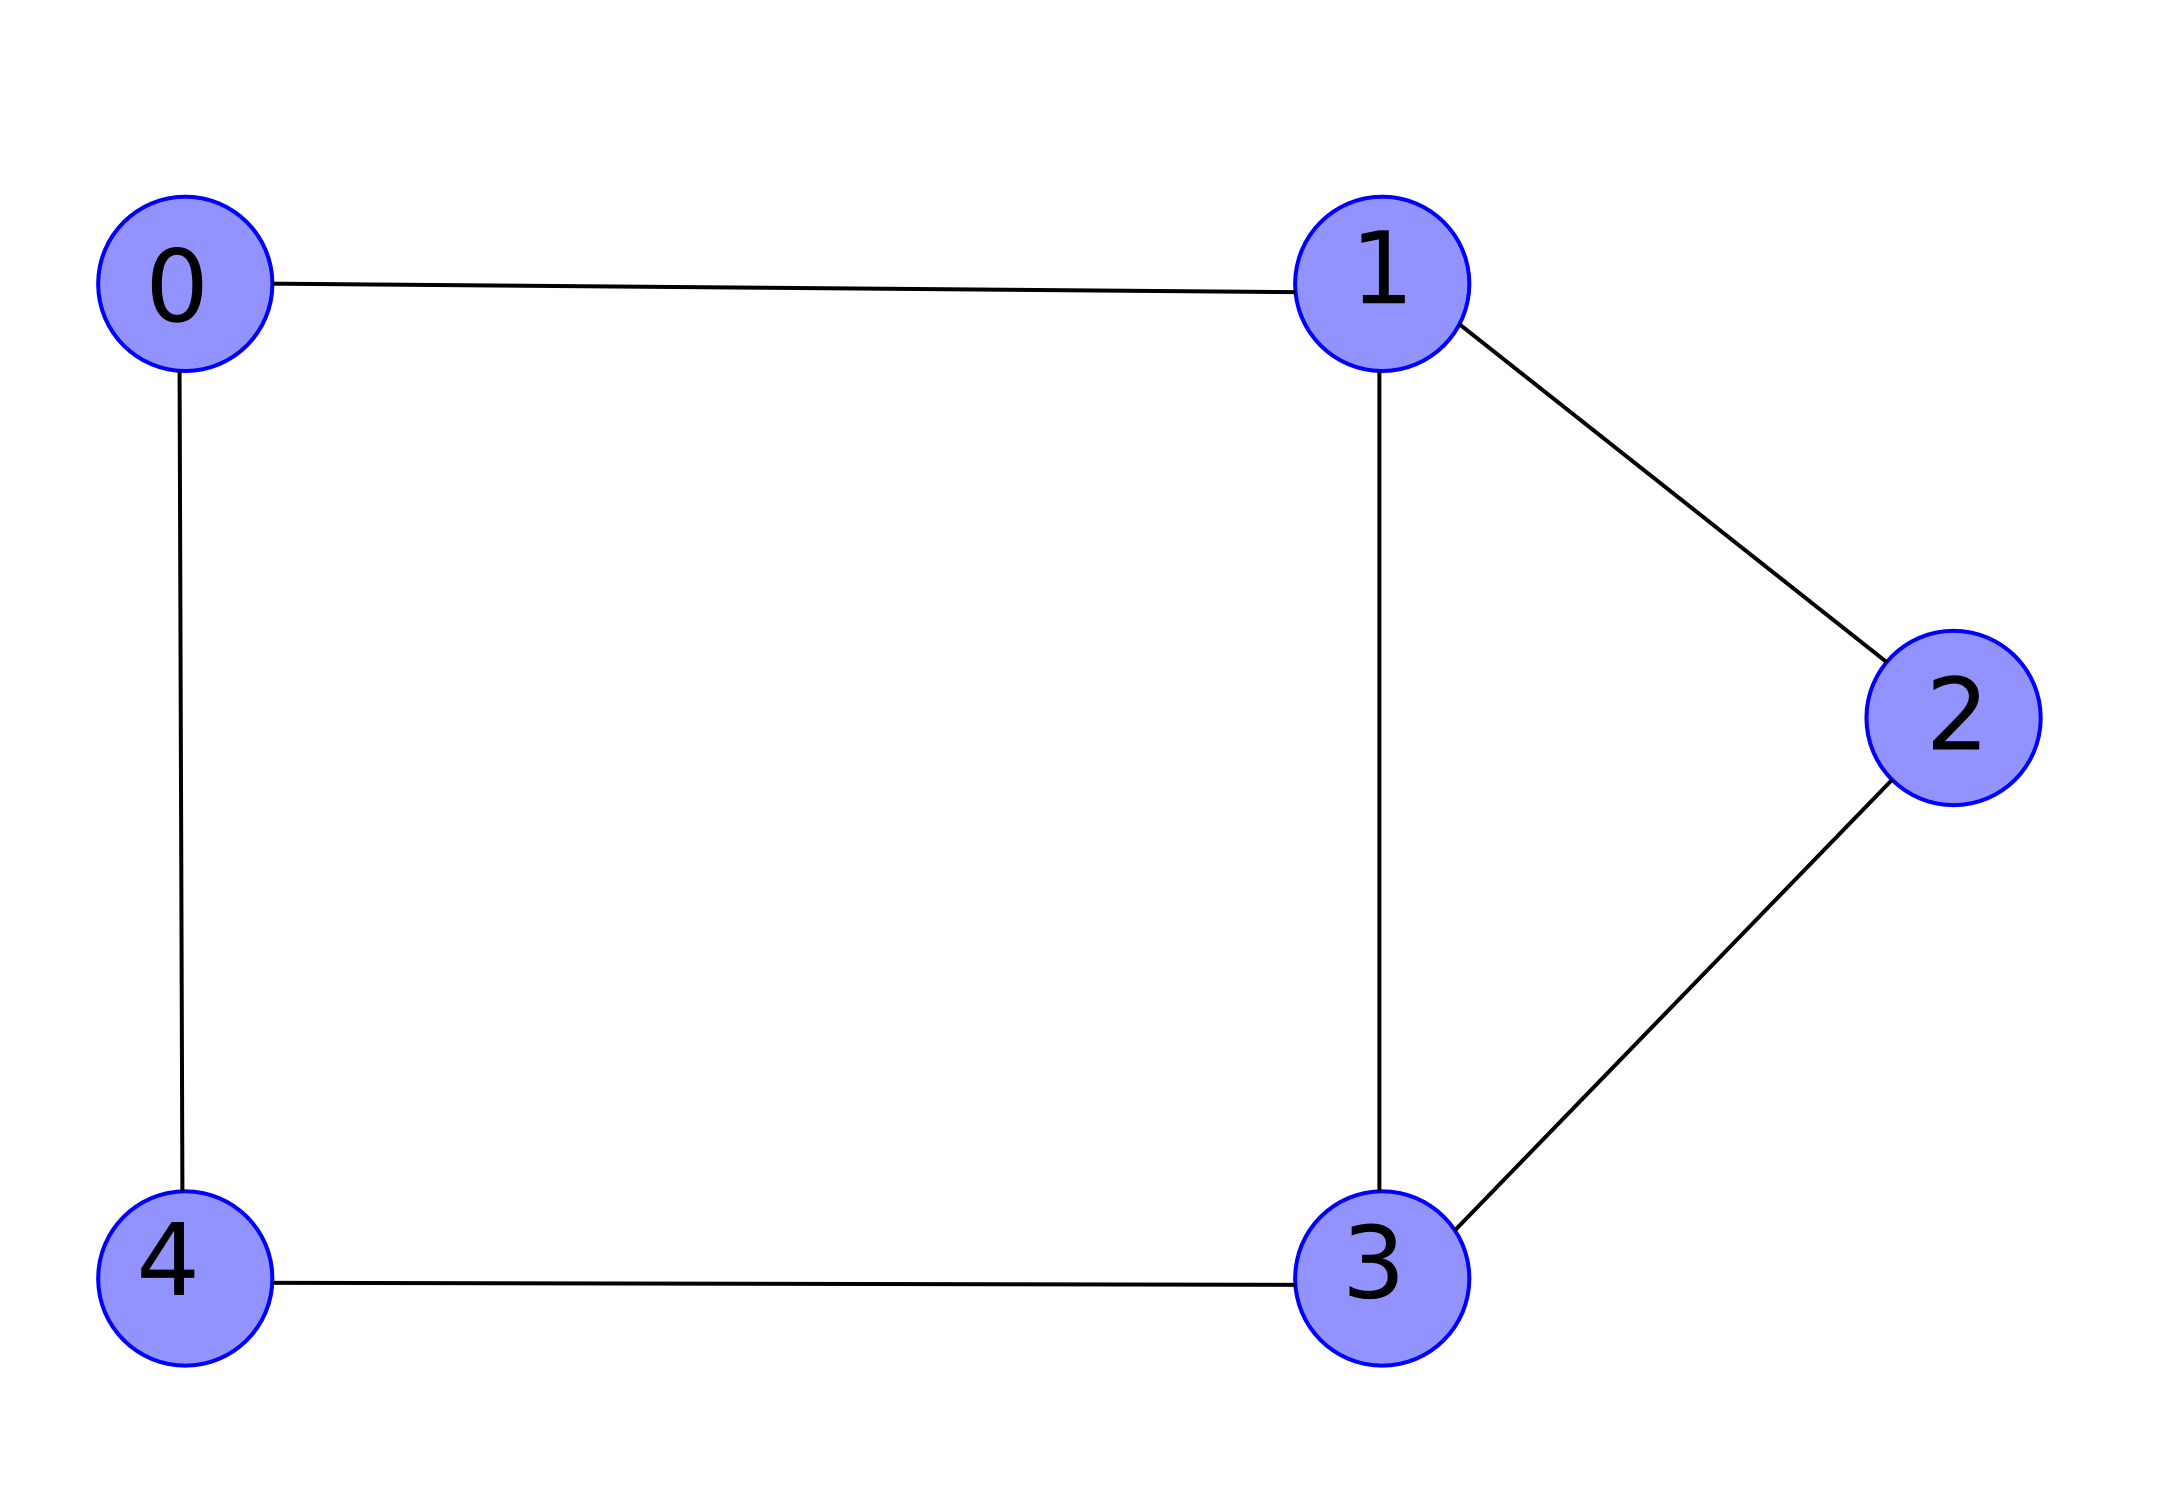
\includegraphics[width=0.3\linewidth]{images/TwoLoops1}
  \caption{A simple graph.}
  \label{fig:TwoLoops1}
\end{figure}

Now consider that we want to find the shortest path ``around the graph'' starting at vertex 0. This question does not map to any graph theoretic terminology. However, we can construct a graph as in Figure \ref{fig:TwoLoops2} which then does have direct mapping to well known graph theory problems. We can repose the question as ````What is the shortest path from vertex 0 to vertex 5?'' and obtain the path we were looking for originally. CORRECTION: There should be an edge (4,5) and NOT and edge (0,5).
\begin{figure}[H]
  \centering
  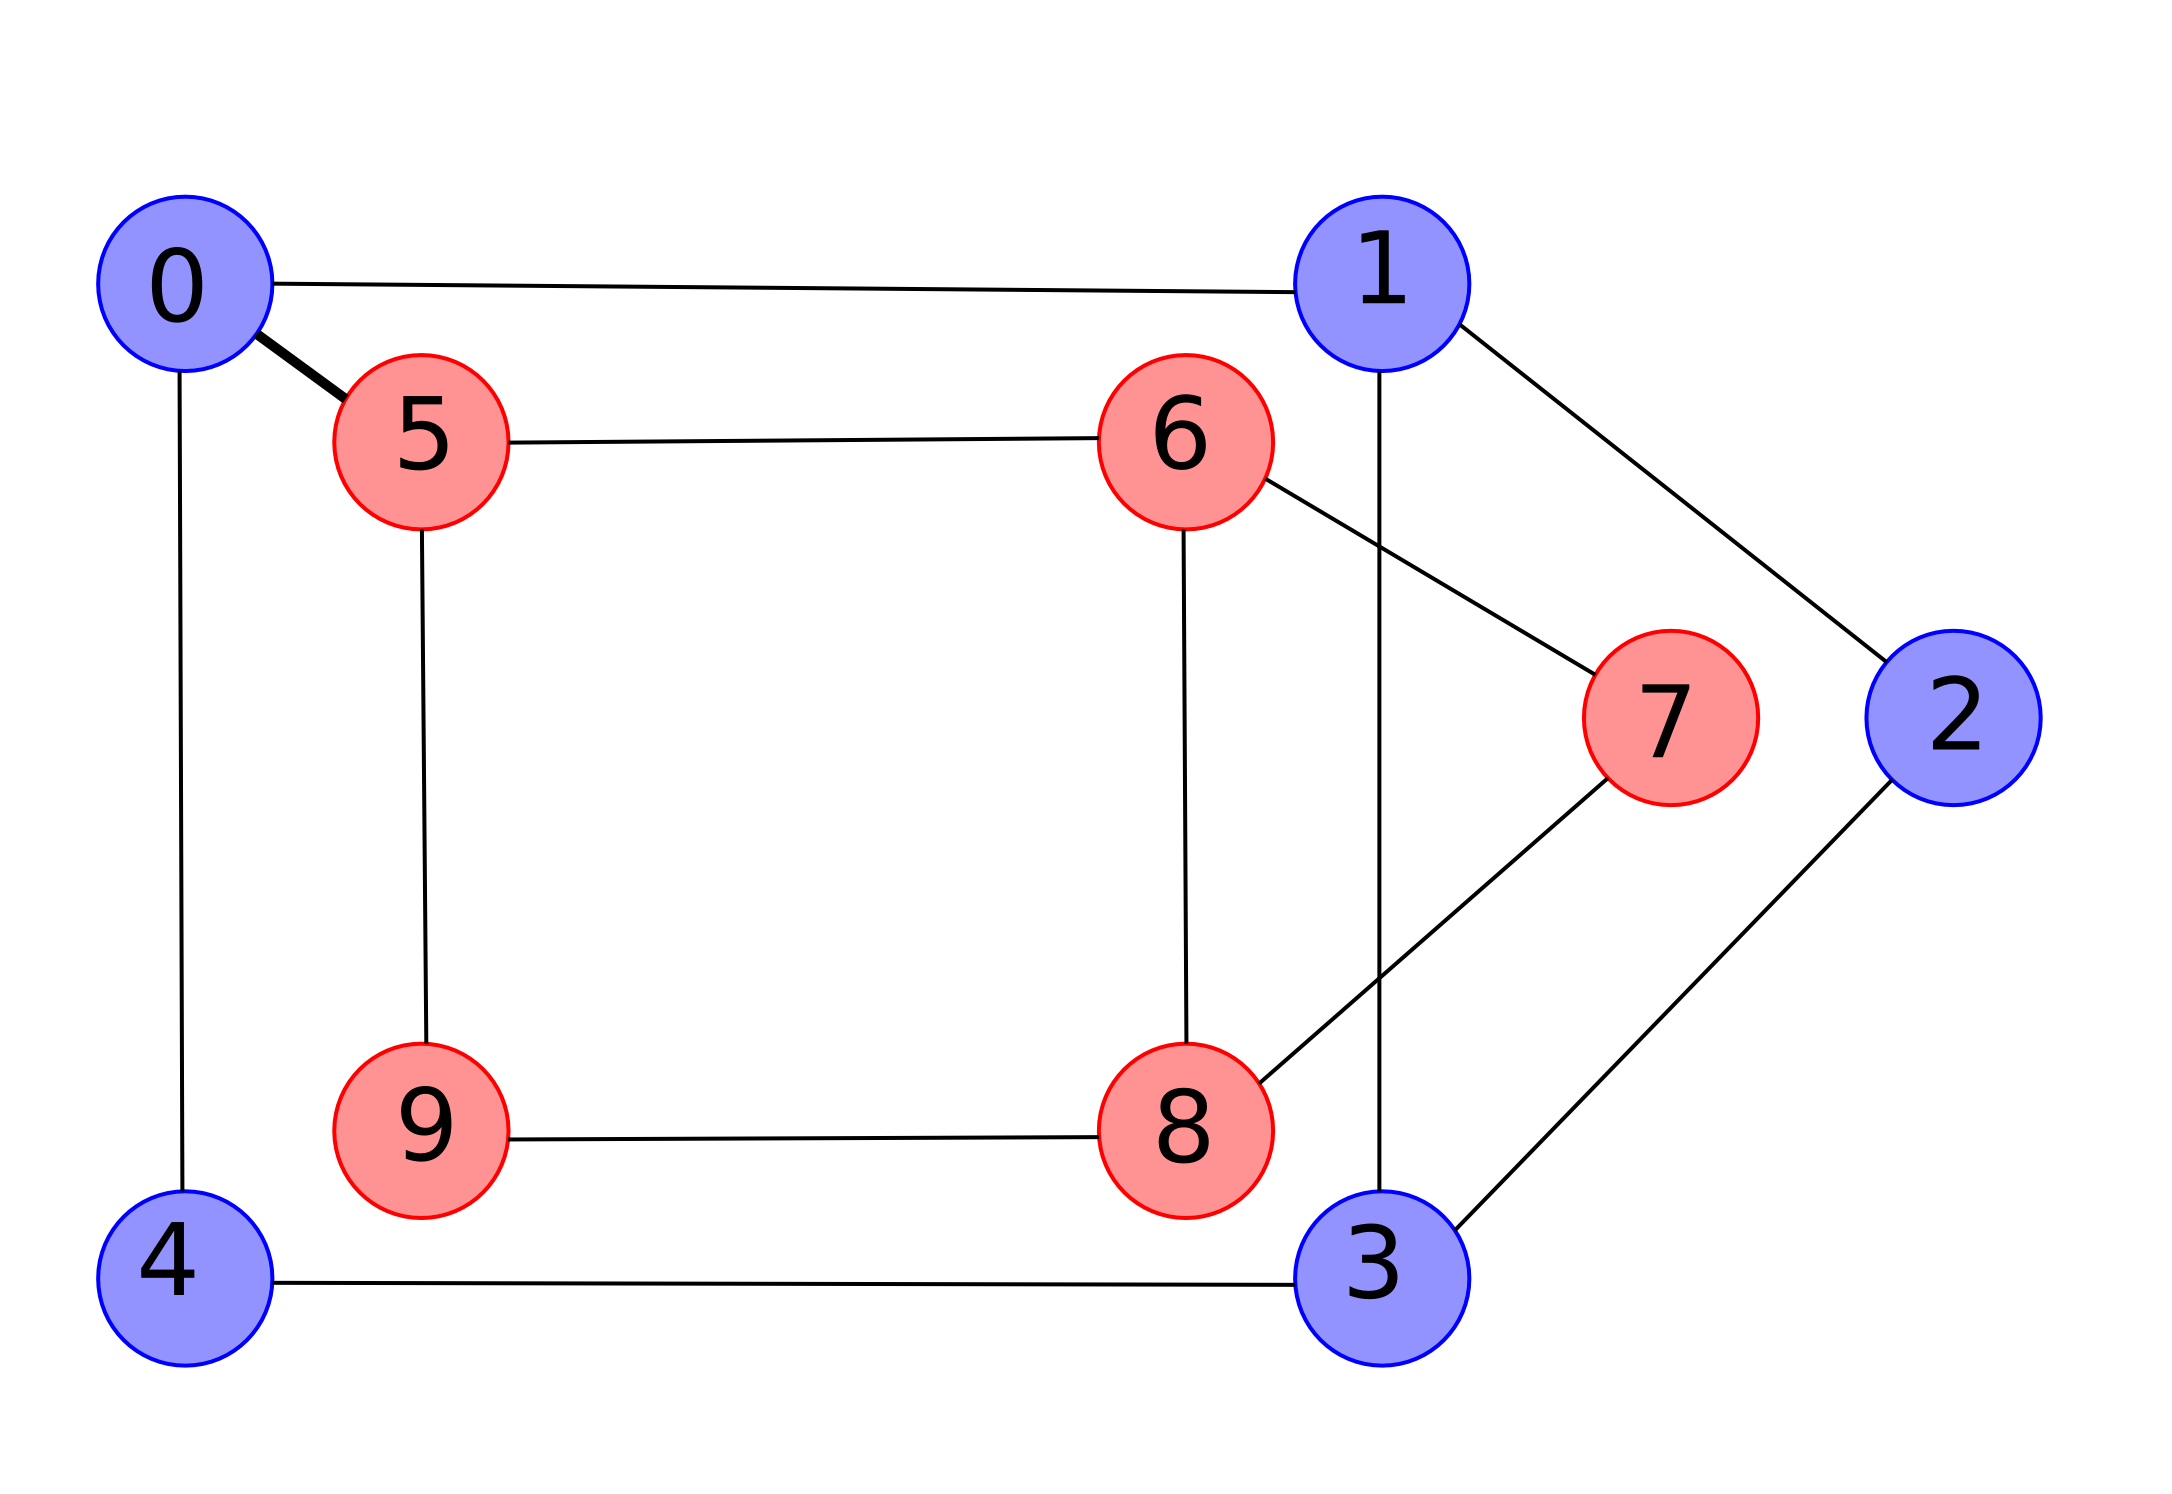
\includegraphics[width=0.3\linewidth]{images/TwoLoops2}
  \caption{The blue vertices and edges are the first loop, while the second loop is shown in red.}
  \label{fig:TwoLoops2}
\end{figure}

To construct this graph, we have simply duplicated all of the vertices, while labeling them with the label $i+N$ where $i$ the original vertex label and $N$ is the number vertices in the original graph.

\subsection{Effect of the Starting Point}
\label{sec:Algorithm:StartingPoint}
To demonstrate why the shortest path must be computed from all starting points and the shortest of those paths chosen for the final output, we have contrived a set of points which clearly demonstrates this phenomenon. Figure \ref{fig:StartingPoint} explains this graphically.

\begin{figure}[H]
\centering
\subfigure[Input contour.]
  {
  
\includegraphics[width=0.22\linewidth]{images/StartingPointDemoGraph}
  \label{fig:StartingPoint:Input}
  }
\subfigure[Potential edges.]
  {
  
\includegraphics[width=0.22\linewidth]{images/StartingPointDemoGraphPotentialEdges}
  \label{fig:StartingPoint:PotentialEdges}
  }
\subfigure[Red: the shortest path from the point not on the square.]
  {
  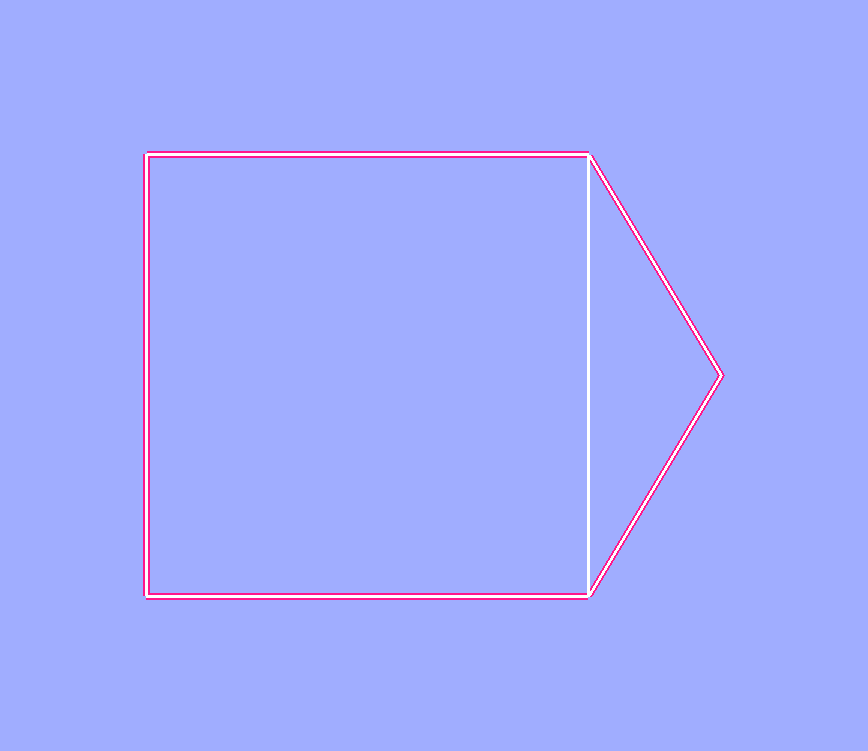
\includegraphics[width=0.22\linewidth]{images/StartingPointDemoGraphShortestPathLong}
  \label{fig:StartingPoint:ShortestPathLong}
  }
\subfigure[Red: the shortest path from any point on the square.]
  {
  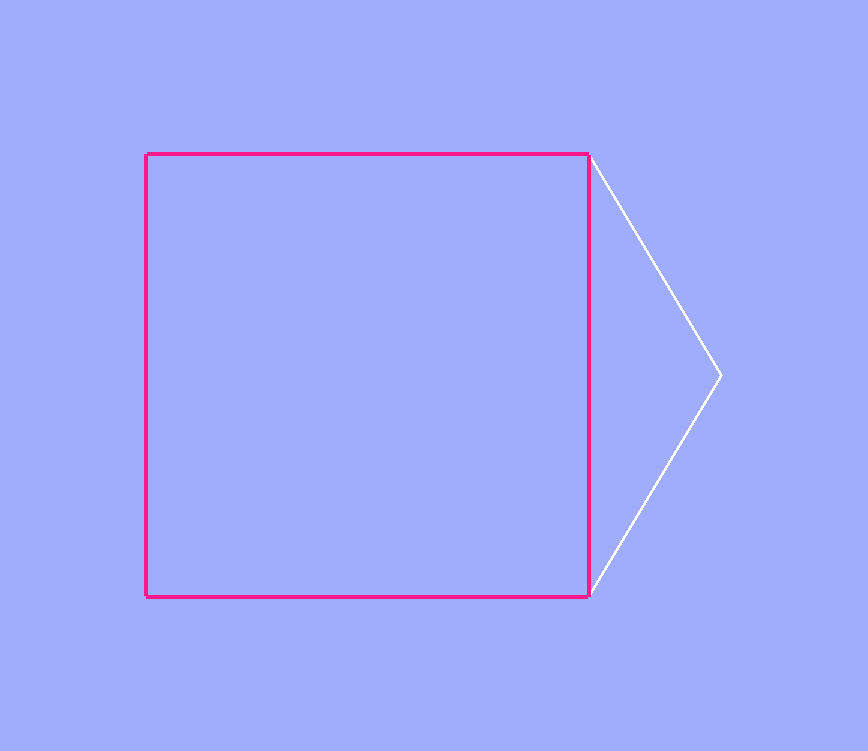
\includegraphics[width=0.22\linewidth]{images/StartingPointDemoGraphShortestPathShort}
  \label{fig:StartingPoint:ShortestPathShort}
  }
\caption{Demonstration of why the starting point is important.}
\label{fig:StartingPoint}
\end{figure}

%%%%%%%%%%%%%%%%%%%%
\section{Demonstration}
\label{sec:Demonstration}
In Figure \ref{fig:NoisyDemo} we show some example simplifications of a noisy input contour. Note that the selection of the StraightnessThreshold can produce significantly varying simplifications.

\begin{figure}[H]
\centering
\subfigure[Simplified contour with StraightnessThreshold = 1.]
  {
  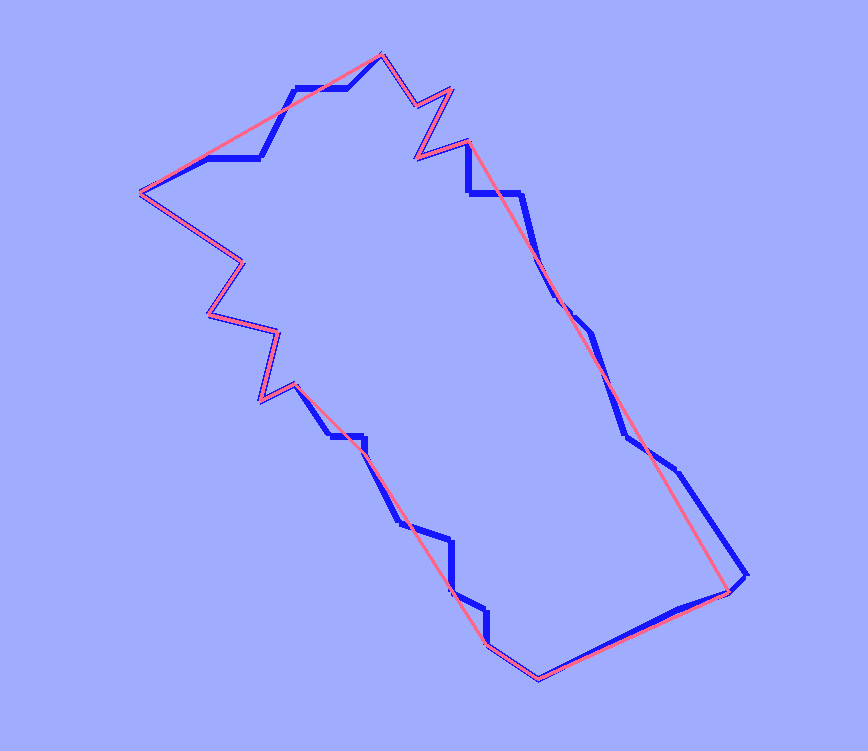
\includegraphics[width=0.3\linewidth]{images/noisy_1}
  \label{fig:NoisyDemo:Straightness_1}
  }
\subfigure[Simplified contour with StraightnessThreshold = 5.]
  {
  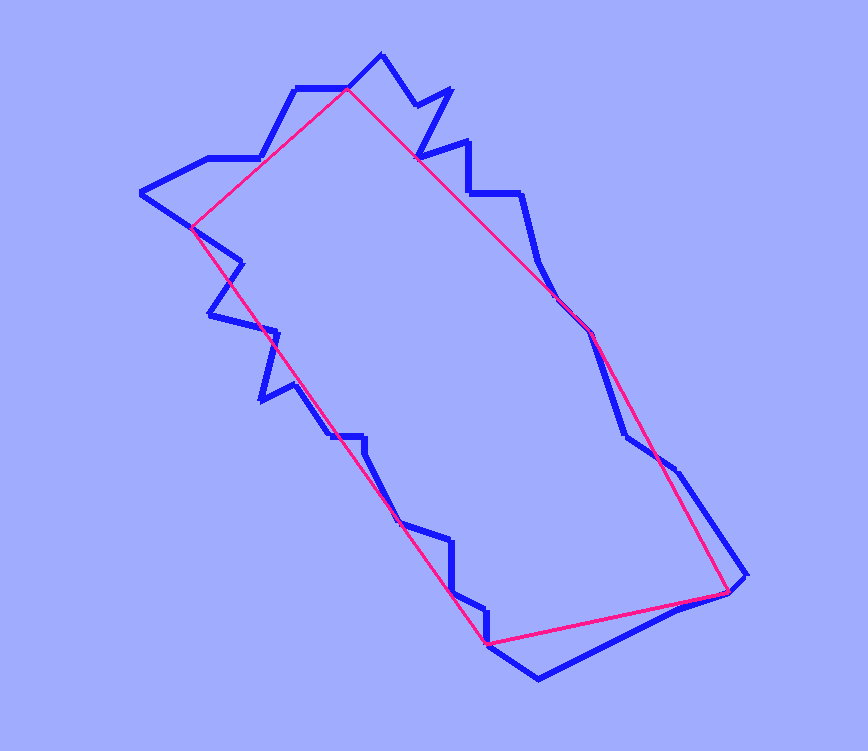
\includegraphics[width=0.3\linewidth]{images/noisy_5}
  \label{fig:NoisyDemo:Straightness_5}
  }
\subfigure[Simplified contour with StraightnessThreshold = 10.]
  {
  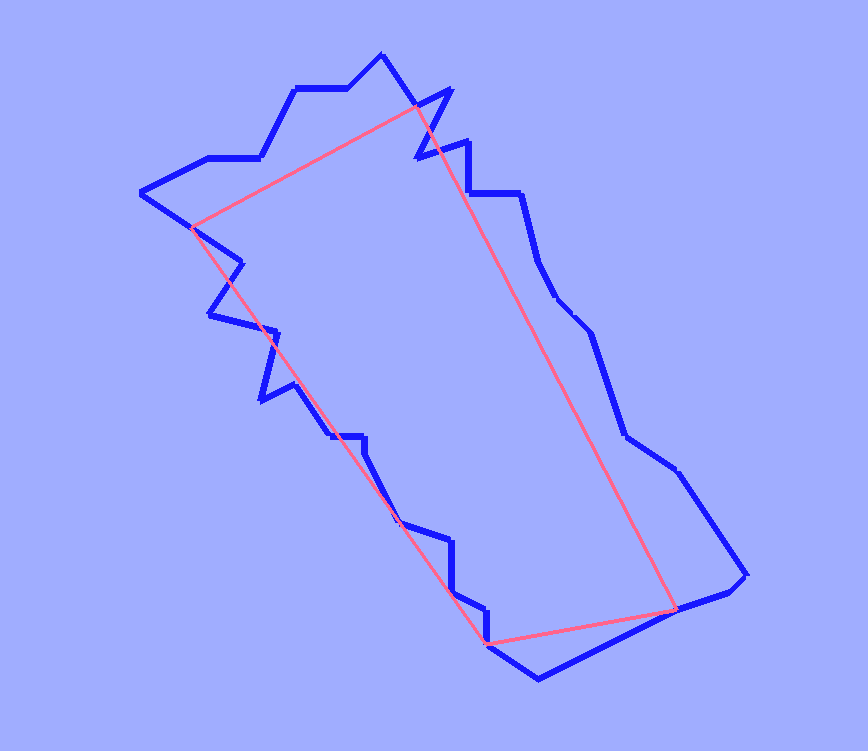
\includegraphics[width=0.3\linewidth]{images/noisy_10}
  \label{fig:NoisyDemo:Straightness_10}
  }
\caption{A noisy input contour and its approximations at StraightnessThreshold = 1, 5, and 10. The input contour is shown in blue, while the simplifications are shown in red.}
\label{fig:NoisyDemo}
\end{figure}


%%%%%%%%%%%%%%%
\section{Code Snippet}

\begin{verbatim}
  vtkSmartPointer<vtkPolyData> inputContour = vtkSmartPointer<vtkPolyData>::New();
  // ... Fill inputContour ...

  vtkSmartPointer<vtkPolyData> simplifiedContour = vtkSmartPointer<vtkPolyData>::New();
  float straightnessErrorTolerance = 1.0;
  OutlineApproximation(inputContour, straightnessErrorTolerance, simplifiedContour);
 
\end{verbatim}

%%%%%%%%%%%
\section{Future Work}
This method requires the selection of a minimum straightness parameter which has a major impact on the resulting simplification. Removing the need to manually specify this parameters would make this algorithm more robust to different data types, as well as provide the best possible results on any particular data set.

%%%%%%%%%%%%%%%
\begin{thebibliography}{9}

	\bibitem{WangThesis}
	  Wang, O.,
	  \emph{Using Aerial Lidar Data to Segment And Model Buildings}.
	  University Of California Santa Cruz Masters Thesis, 2006


	\bibitem{WangPaper}
	  Wang. O, Lodha. S, Helmbold, D.,
	  \emph{A Bayesian Approach to Building Footprint Extraction from Aerial LIDAR Data}.
	  3D Data Processing, Visualization, and Transmission 2006

\end{thebibliography}

\end{document}